\label{chap:differential-evolution}
In the first part of the chapter we make an overview to Differential Evolution, moving later to the mutation and crossover strategies that we have used to evolve the NRAM controller and finishing with the DENN overview.

\section{Differential Evolution}
Differential Evolution (DE) is a metaheuristic\footnote{A metaheuristic is a procedure that has as objective the search, creation or selection of an heuristic that could be find a optimal solution of a problem.} introduced in \cite{DESEHGOCS:1997}, belonging to the family of Evolutionary Algorithm (EA), that has as objective the solution searching through the parallel evolution of a set of candidate solutions. 

Differential Evolution is a parallel iterative direct search metaheuristic which utilizes NP D-dimensional numerical vectors 
\begin{center}
	\begin{equation}
		x_{i, G},\ i=1,\ \dots,\ NP 
	\end{equation}
\end{center}
called \textbf{population}, where each of them is called \textbf{individual}, that are manipulated for \textbf{G} generation, where the NP are not reduced nor incremented, in searching of an individual that can be considered as solution given an objective. This objective, as for the gradient based optimization algorithms, is represented by a function called in this case \textbf{fitness function} that represented the goodness of an individual and do. For a better exploration of a solution, the individuals must be randomly initialized covering the entire parameters space. 

As stated previously, the algorithm go on for G generation where in each of these are generated three set of individuals called, respectively, \textbf{targets}, \textbf{donors} and \textbf{trials}. The targets set is formed by individual which are selected for the creation of donors set, called also mutant. Once the mutants are generated, targets and donors sets are mixed up with some crossover strategy creating finally the trials set. Following the latter is used for the creation of next generation targets set. \\

\begin{figure}[t]
	\centering
	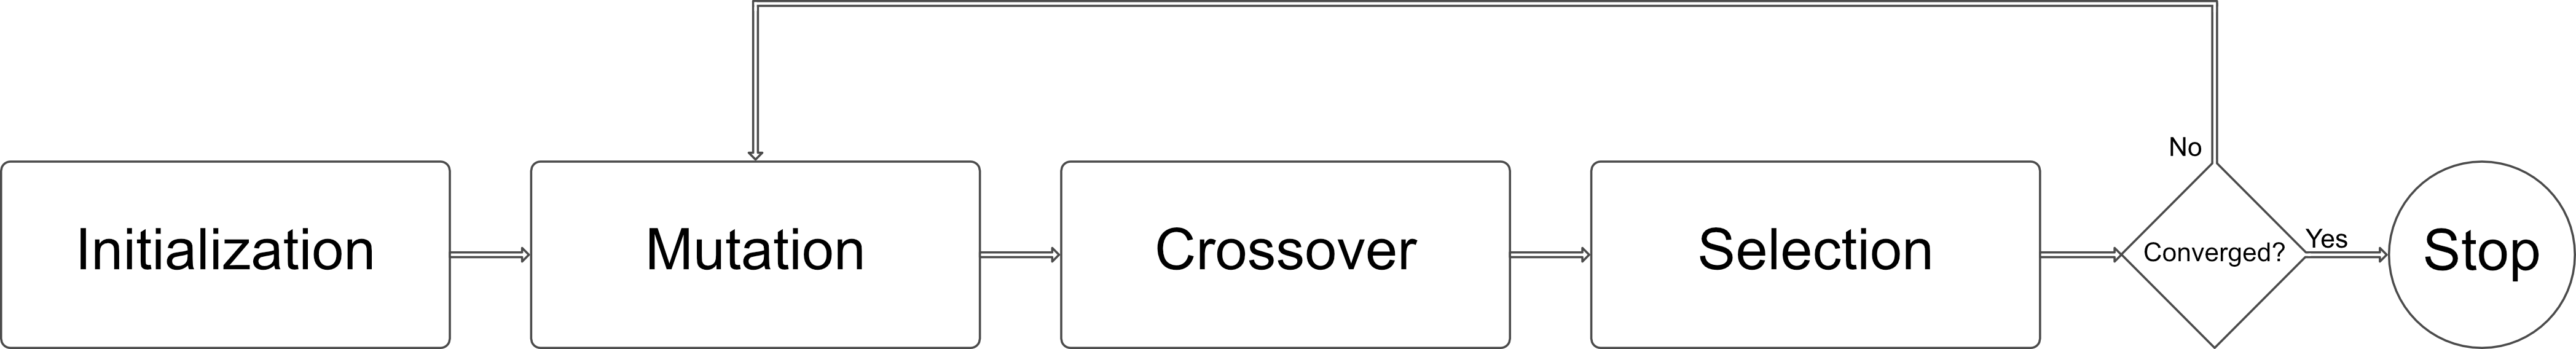
\includegraphics[width=\textwidth]{figures/de-flow.png}
	\caption{Differential Evolution flow diagram.}
\end{figure}

Summing up, after the targets set initialization, the step executed in every DE generation are:
\begin{itemize}
	\item{\textbf{Mutation}: Let target $x$ at the generation $G$, a mutant is generated combining $x$ through a summation with some others targets combined with some strategy and scaled through a global real valued user defined constant $F$. As example, with the strategy \textbf{rand/1} introduced in \cite{DESEHGOCS:1997} we have
	\begin{center}
		\begin{equation}
			v_{i,G+1} = x_{r_{1},G} + F\cdot(x_{r_{2},G} - x_{x_{3},G})
		\end{equation}
	\end{center}
	where $r_{1},r_{2},r_{3} \in \{1,2,\dots,NP\}$ and must be each other different.}
	\item{\textbf{Crossover}: Because the mutation itself could leads to the creation of equal mutants, this step is introduced. As stated previously, the crossover does nothing else than mixing up the targets with the mutants (donors) with some strategy, generating the trials. For example, let the target vector $x_{i,G}$ and the mutant $v_{i,G+1}$ the \textbf{bin} strategy work as follows
	\begin{equation}
		u_{ji, G+1} = \begin{cases}
			v_{ji,G+1}, & \textrm{if}\ (\textit{randb}(j) \leq \textit{CR})\ \textrm{or}\ j=\textit{rnbr}(i)\\
			x_{ji,G}, & \textrm{if}\ (\textit{randb}(j) > \textit{CR})\ \textrm{and}\ j\neq\textit{rnbr(i)}
		\end{cases}
	\end{equation}
	for $i=1,2,\dots,D$. The function $\textit{randb}(j)$ generate a real valued number for the $j^{th}$ parameter according to binomial distribution, $\textrm{CR}\in[0,1]$ is the global user defined crossover constant used as a threshold and $\textit{rnbr}(i)$ is a function that generate randomly an index which ensures that is selected at least one parameter of the mutant $v_{i}$.}
	\item{\textbf{Selection}: After the trials set is generated is made a comparison respect to the donors set for each vector, i.e. the donor $x_{i, G}$ is compared respect to the trial $u_{i,G+1}$ using the cost function. Hence, if the donor have a smaller cost respect to the trial, than it is retained for the next generation donors set and vice-versa.}
\end{itemize}

During the algorithm explanation is introduced one strategy both for the mutation and crossover step, but they are not the unique even regard the optimization algorithm. Hence, in order to classify all the variants it's used the notation $DE/x/y/z$ where:
\begin{itemize}
	\item{\textbf{DE}: indicates the used optimization algorithm;}
	\item{\textbf{x}: indicates the mutation strategy;}
	\item{\textbf{y}: indicates how many targets couple are selected in the mutation step;}
	\item{\textbf{z}: indicates the crossover strategy;}
\end{itemize}
Hence, for example, a possible variant is \textit{DE/rand/1/bin}. For the thesis work have been used and tested DE's different configurations made available by the framework DENN (\ref{sec:DENN}). Hence, about this following are introduced some of the used algorithms and strategies.
\subsection{Differential Evolution variants}
\subsubsection{Adaptive DE (JADE)}
The base version of Differential Evolution is powerful, but one of its biggest drawback is that the constants $F$ and $CR$ are leave to the user decision. Though is suggest in \cite{RPODE:2005} to set the $F\in[0.4, 0.95]$ and $CR \in (0, 0.2)$ if the function is separable and $CR \in (0.9, 1.0)$ when the function's parameters are dependent, remain always the fact that are problem dependent. 

Hence trying to resolve this problem in \cite{JADE:2009} is introduced JADE. Briefly, this DE variant lift the user from the duty of selecting the best combination of $F$ and $CR$ constant. This is done with a parameter adaptation system that search the constants best values refining them for each generation. Moreover, these constants are generated for each individual and so they are, generally, different one from the another, e.g. $\textit{CR}_{1} \neq \textit{CR}_{i}$. Formally what is done is the following:
\begin{itemize}
	\item{\textbf{CR}: Let $\mu_{\textit{CR}}$ the \textit{CR}'s mean, initialized previous the first generation to $0.5$. For each generation the crossover probability $\textit{CR}_{i}$ associated to the $x_{i}$ individual, is generated according to a normal distribution with mean $\mu_{CR}$ and a standard deviation $0.1$
	\begin{center}
		\begin{equation}
			\textit{CR}_{i} = \textrm{randn}_{i}(\mu_{\textit{CR}}, 0.1)
		\end{equation}
	\end{center}
	truncated respect to the interval $[0, 1]$. 
	
	
	After the generation ending the best $\textit{CR}_{i}$s, i.e. the \textit{CR}s associated to the trials $v$ better than the targets $x$, are added to the set $S_{\textit{CR}}$, i.e. the set containing the $\textit{CR}_{i}$ that is successful. After this, the mean $\mu_{\textit{CR}}$ is recalculated as follows:
	\begin{center}
		\begin{equation}
			\mu_{\textit{CR}} = (1 - c)\cdot\mu_{\textit{CR}} + c\cdot\textrm{mean}_{A}(S_{\textit{CR}})
		\end{equation}
	\end{center}
	where the $c$ is a positive constant between 0 and 1 and $mean_{A}(\cdot)$ is the arithmetic mean.	
	}
	\item{\textbf{F}: similarly to CR, \textit{F} is generated for each target with a system similar to that used for CR. Let $\mu_{F}$ the F's mean, initialized previous the first generation to $0.5$. Hence, for each generation and for each target individual, is generated a $F_{i}$ using the mean $\mu_{F}$ and a standard deviation $0.1$ as follows:
		\begin{center}
			\begin{equation}
				F_{i} = \textrm{randc}_{i}(\mu_{F}, 0.1)
			\end{equation}
		\end{center}
		that is truncated if $F_{i} > 1$ and regenerated if $F_{i} \leq 0$, so that a $F_{i} \in (0, 1]$ and $\textrm{randc}_{i}$ is a Cauchy random generator associated to each target individual.
		
		As for the CR case, denoting $S_{\textit{F}}$ the set of successful mutation factors, to which are added the successful Fs at the end of a generation. Then for each generation the mean $\mu_{F}$ is generated as follows:
		\begin{center}
			\begin{equation}
				\mu_{F} = (1 - c)\cdot\mu_{F} + c\cdot\textrm{mean}_{L}(S_{F})
			\end{equation}
		\end{center}
		where the $c$ is also here a positive constant in $[0, 1]$ and $\textit{mean}_{L}$ is the Lehmer mean defined as:
		\begin{center}
			\begin{equation}
				\textrm{mean}_{L}(S_{F}) = \frac{\sum_{F \in S_{F}}F^{2}}{\sum\limits{F \in S_{F}}F} 
			\end{equation}
		\end{center}
		}
\end{itemize}

Moreover, JADE has introduced an optional external memory denoted as \textbf{A} with size equal than \textit{NP}, where is stored all the targets that have failed the selection process. Once the memory is full and is necessary adding a new one, an individual is randomly deleted.

\subsubsection{Success-History based Adaptive DE (SHADE)}
The JADE's main problem is that the generation of $\textit{CR}_{i}$ and $F_{i}$ is controlled by the memories $S_{\textit{CR}}$ and $S_{F}$, that for how are managed could contain poor settings of $\textit{CR}$ and $F$. Hence, this fact can leads JADE to have degraded performance. 

SHADE introduced in \cite{SHADE:2013} aims to increment the robustness of JADE introducing an alternative system of crossover and mutation constants generation.

\subsubsection{L-SHADE}

\subsection{Mutation strategies}

\subsubsection{Rand}

\subsubsection{Best}

\subsubsection{DEGL} % Rename with the true name

\subsubsection{Current to pbest}\label{subsubsec:curr_p_best}

\subsection{Crossover strategies}

\subsubsection{Bin}

\subsubsection{Exp}

\begin{figure}[h!]

	\begin{tikzpicture}[smooth]
		\begin{axis}[
  			axis x line=center,
  			axis y line=center,
  			xlabel={$x1$},
  			ylabel={$x2$},
  			xlabel style={below right},
  			ylabel style={above left},	
		    xmin=0, xmax=1,
		    ymin=0, ymax=1,
			legend pos=north east  			
		]
  			\addplot[mark=none, black] table{data/differential-evolution-space.txt};
 		\end{axis}
	\end{tikzpicture}
	\caption{}
	\label{fig:mutant-generation-plot}
\end{figure}
		

\section{DENN}\label{sec:DENN}